\section{String instruments}
\bi

\i This section provides an introduction to 
the production of sound by string instruments.

\i We will consider the harp, guitar, and violin
to illustrate the fundamental differences between
string instruments.

\i We will follow the presentation in the book 
``How music works," by John Powell.
More details can be found in the text by Berg and Stork.

\ei
%%%%%%%%%%%%%%%%%%%%%%%%%%%%%%%%%%%%%%%%%%%%%%
\subsection{Sounds from strings}
\bi

\i String instruments come in two basic types: 
those that are plucked and those that are bowed.

\i Examples of plucked string instruments are the 
harp, guitar, banjo, ...
Examples of bowed string instruments are the 
violin, cello, ...

\i Plucking and bowing are the two basic 
methods for exciting vibrations in a stretched string.

\i As discussed in a previous section,
the frequency of a standing wave vibration of a 
stretched string depends on only three things:
(i) the length of the string, 
(ii) what the string is made of, and
(iii) the tension in the string.

(i) The length of the string determines how far
the waves have to travel to go from one end to
another.
The longer the string, the longer the travel
time, and hence the lower the frequency of vibration.

(ii) What the string is made of is important 
since heavier strings offer more resistance 
to changes in their state of motion, and hence 
correspond to lower-frequency waves.

(iii) The tension in the string is a measure of 
how tightly the string is stretched.
Strings under higher tension are pulled back toward
their equilibrium position with greater restoring
force, and hence correspond to higher-frequency waves.

\i The mathematical formula for the frequency
of the nth standing wave vibration is
%
\be
f_n = \frac{n}{2L}\sqrt{\frac{F}{\mu}}\,,
\qquad
n=1,2,3,\cdots
\ee
%
where $L$ is the length of the string,
$\mu$ is its mass per unit length, and 
$F$ is the tension in the string.
($f_1$ is the fundamental frequency and 
$f_n = nf_1$ is the nth harmonic.)

\i A vibrating string by itself doesn't produce 
much sound.
The vibrations of a string need to be amplified 
by attaching them to some sort of wooden box 
(called a soundboard), 
which is able to drive more air and produce a louder sound.

\i The interaction between the natural frequencies 
of the strings and the natural frequencies of the 
soundboard are responsible for the rich timbre of the
different string instruments.

\ei
%%%%%%%%%%%%%%%%%%%%%%%%%%%%%%%%%%%%%%%%%%
\subsection{Physics of a plucked string}
\bi

\i Where you pluck a string determines the timbre
of the sound produced by the subsequent vibration.

\i As shown in Figure~\ref{f:pluckedstrings},
plucking a string in the middle give the 
purest tones, consisting of just the odd harmonics.
Plucking a string near the ends produces 
``fuller" tones, with contributions from both even 
and odd harmonics.
%
\begin{figure}[htbp]
\begin{center}
\begin{tabular}{cc}
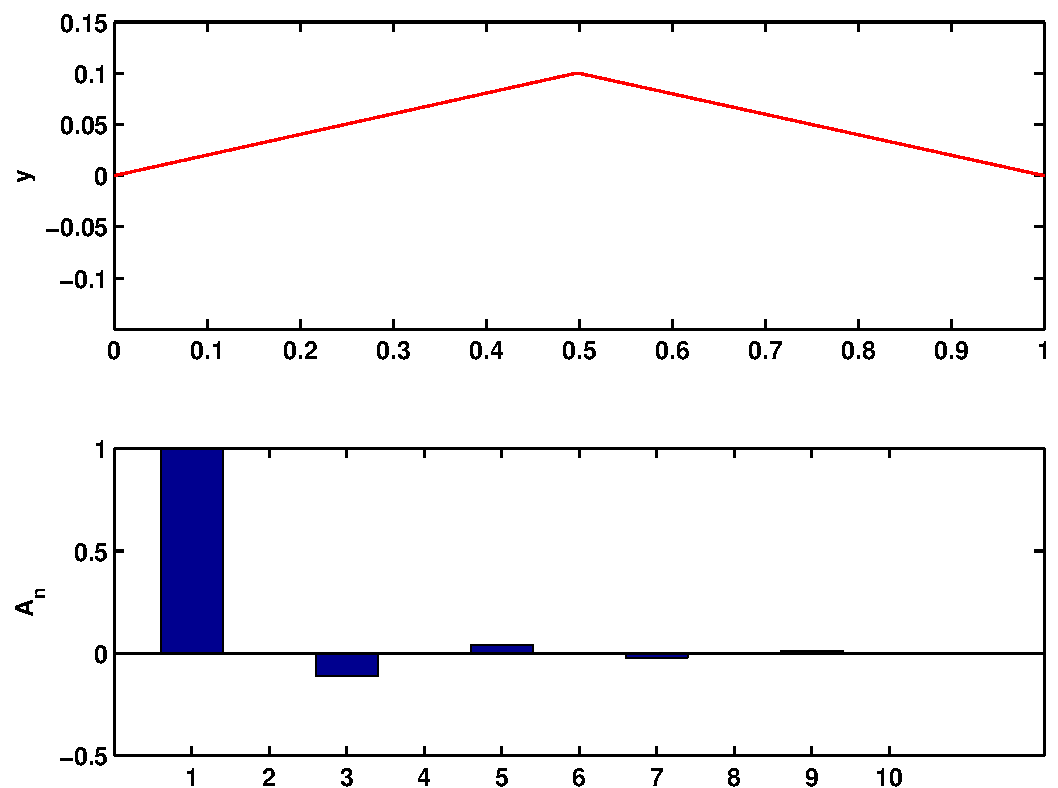
\includegraphics[width=.5\textwidth]{pluckedstringharmonics1_2.pdf} &
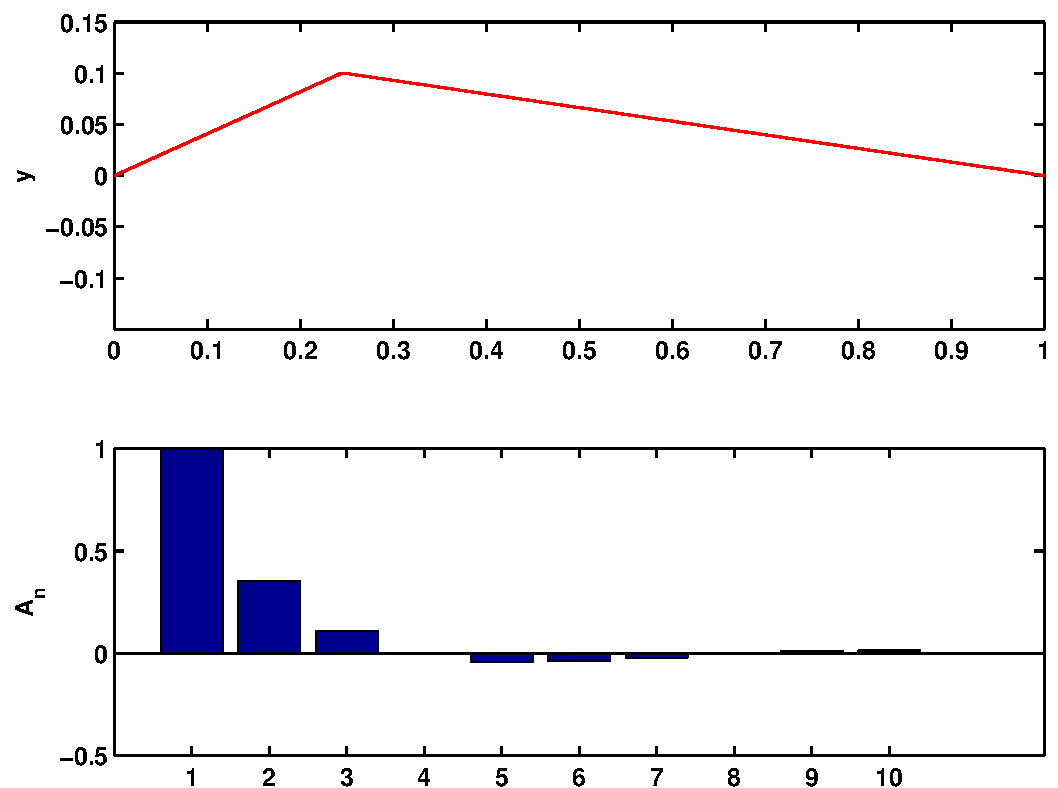
\includegraphics[width=.5\textwidth]{pluckedstringharmonics1_4.pdf}
\\
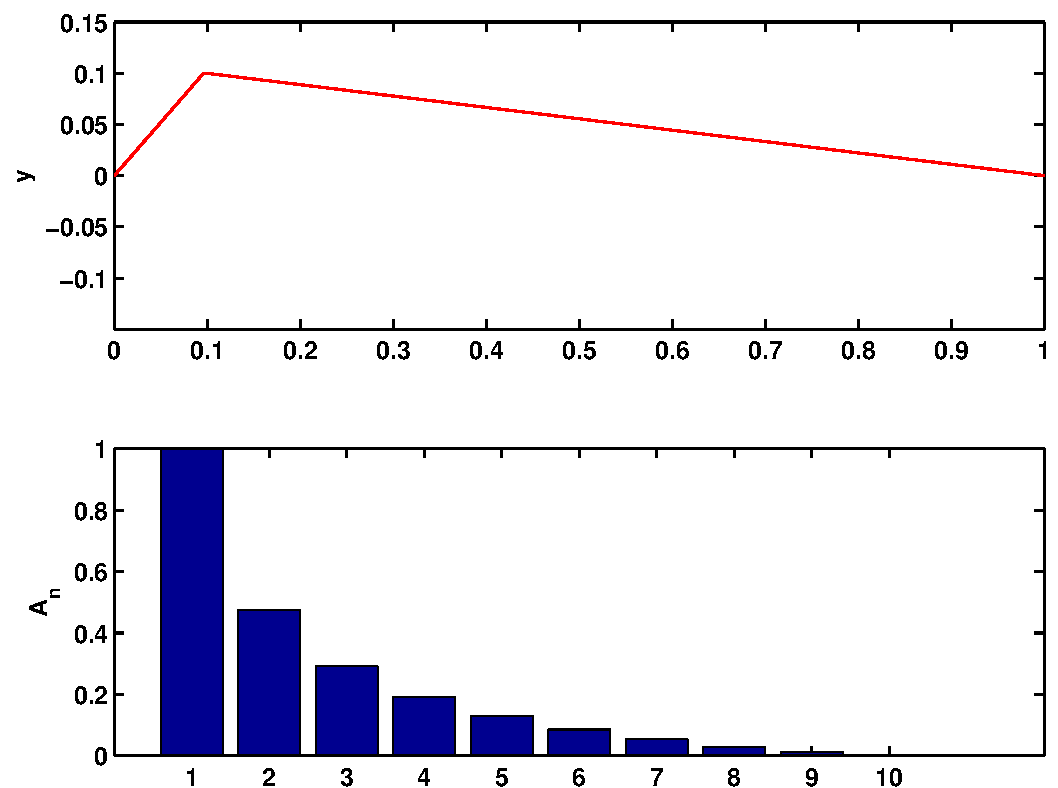
\includegraphics[width=.5\textwidth]{pluckedstringharmonics1_10.pdf} &
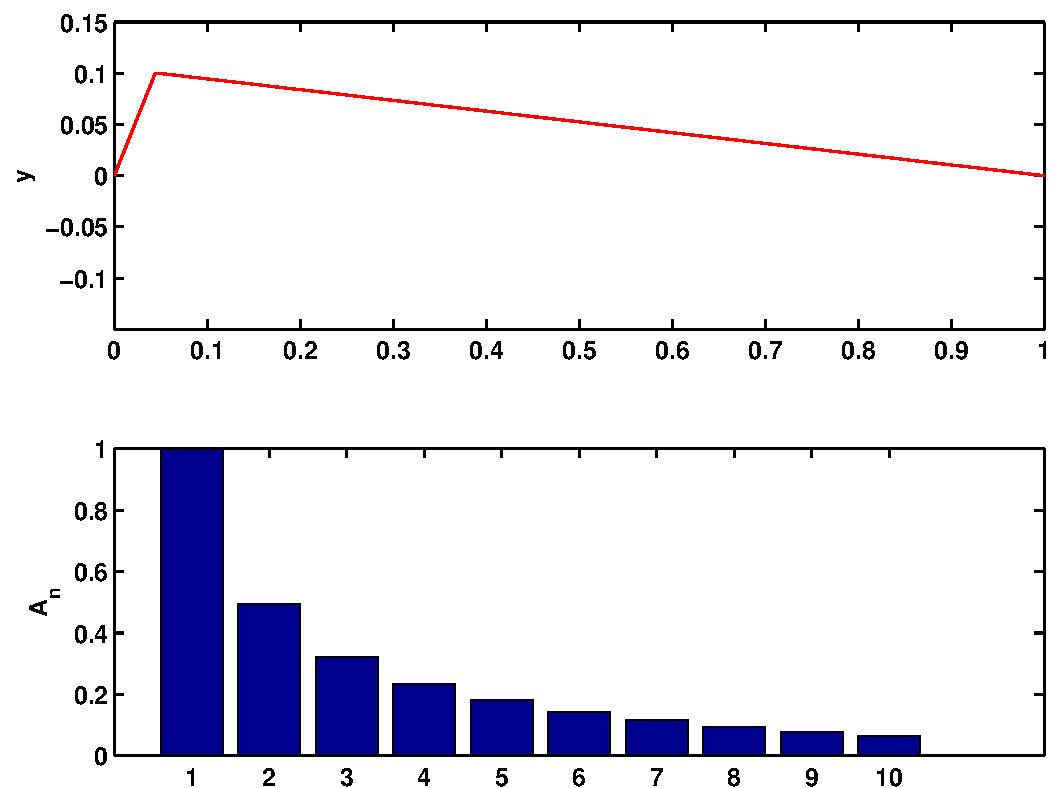
\includegraphics[width=.5\textwidth]{pluckedstringharmonics1_20.pdf} 
\end{tabular}
\caption{Fourier coefficients corresponding to strings
plucked in different locations.
Note that a string plucked in the center (top-left plot)
corresponds to the purest tone, with small contributions 
from just the odd harmonics.
A string plucked near the end (bottom-right plot) corresponds
to a fuller sound, with relatively large contributions from 
many harmonics.}
\label{f:pluckedstrings}
\end{center}
\end{figure}

\i \demo Reproduce some of these plots using the matlab
routine {\tt pluckedstringharmonics.m} for different
values of the plucking location $\alpha$.

\i \demo Watch the YouTube videos:\\
``Motion of a plucked string"
{\tt http://www.youtube.com/watch?v=\_X72on6CSL0} and\\
``Guitar Oscillations Captured with iPhone 4"
{\tt http://www.youtube.com/watch?v=TKF6nFzpHBU}.

\i Note that the guitar string oscillations captured 
with an iPhone show the {\em same wave} pulse at 
different locations along the string.
(So this is {\em not} how a real wave looks on a guitar string.)
This is due to the {\em rolling shutter} feature of 
the iPhone video camera, which opens parallel to the 
longer side of the iPhone.
If the iPhone was positioned such that the longer 
side of the iPhone was parallel to the guitar strings,
then one wouldn't see these wave pulses at all.

\i \demo Verify these statements using a guitar
and an iPhone.
(Note: To see the wave pulses, the strings need to
be brightly lit---e.g., use a flood light placed
next to the strings if you are doing this indoors.
A bright light increases the iPhone frame rate
to 30 frames per second.)

\i Mathematically, the Fourier coefficients for a plucked 
string are proportional to 
$\sin(n\pi\alpha)/n^2$, where $n=1,2,\cdots$,
and $\alpha$ is the fractional distance from the bridge
(i.e., where the string is plucked).

\i Note that if $\alpha = 1/N$, then there is 
no contribution from the Nth harmonic and its multiples.

\i For a plucked string, the sideways force on 
the bridge has the shape of a square wave.
The relative durations of the positive and negative 
parts of the square wave depend on $\alpha$.
The Fourier coefficients for this type of square 
wave are proportional to $\sin(n\pi\alpha)/n$.

\i \demo Illustrate this using the matlab
routine {\tt pluckedstring.m}
for different values of the plucking location $\alpha$.

\ei
%%%%%%%%%%%%%%%%%%%%%%%%%%%%%%%%%%%%%%%%%%
\subsection{Physics of a bowed string}
\bi

\i Bowing is another way to excite the vibrations
of a stretched string.

\i The violin, cello, and bass are examples of bowed string
instruments.

\i A bow is typically made from hairs from a horse's tail, 
stretched tight on a stick.
The horse hairs are made sticky by rubbing them with rosin
(dried tree resin).

\i The bow excites vibrations in a string via an 
alternating {\em stick-slip} motion.
The bow first `sticks' to a string, dragging it 
away from its equilibrium position.
The string then `slips' from under the bow,
moving back towards, and then overshooting, 
its equilibrium position (Figure~\ref{f:stickslip}).
%
\begin{figure}[htbp]
\begin{center}
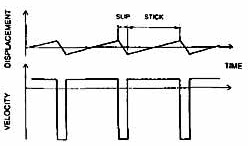
\includegraphics[width=.6\textwidth]{stickslip.jpg}
\caption{Stick-slip motion of a bowed string.
Top panel shows string displacement as a function of time.
Bottom panel shows string velocity as a function of time.
This example is for the case where the string is bowed
one-quarter of the way from the bridge.
(Figure taken from {\tt http://www.zainea.com/}.)}
\label{f:stickslip}
\end{center}
\end{figure}

\i This stick-slip motion happens hundreds of times per 
second, aligning itself with the natural vibrational 
frequency of the string.

\i \demo 
Wet your finger and rub it across a window pane 
or rim of a glass.
Your finger tip slips and sticks as you press 
your finger against the glass, producing a 
squeaking sound as it moves.

\i The vibrational motion of a bowed a string 
is basically a triangular wave that runs around
a parabolic arc, as shown in Figure~\ref{f:violinbowed}.
%
\begin{figure}[htbp]
\begin{center}
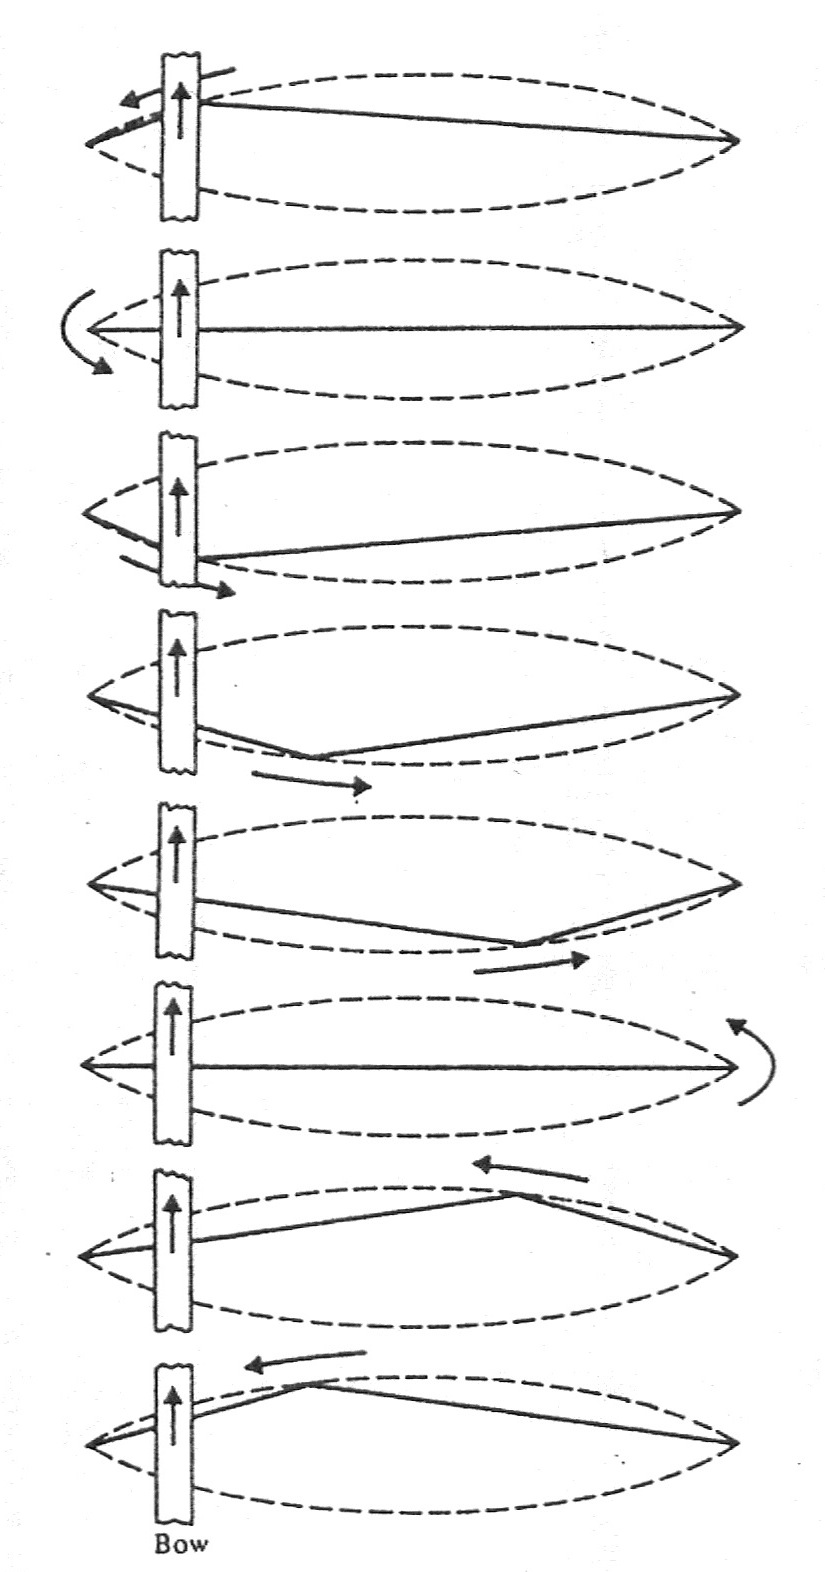
\includegraphics[height=.8\textheight]{violinbowed.jpg}
\caption{Schematic diagram showing the motion of a bowed string.
In the top three panels, the string slips from underneath 
the bow, with the kink traveling counter-clockwise
from bow to bridge to bow again.
In the bottom five panels, the string sticks to the bow 
and is dragged along with it, with the kink traveling 
counter-clockwise from bow to nut, and eventually back to 
the bow again.
The envelope of the motion consists of two parabolic arcs.
(Figure taken from {\tt http://www.colorado.edu/physics/phys1240/}.)}
\label{f:violinbowed}
\end{center}
\end{figure}

\i \demo
Watch the YouTube video
``Bowed violin string in slow motion"\\
{\tt http://www.youtube.com/watch?v=6JeyiM0YNo4}.

\i It turns out that {\em all} the harmonics of 
the vibrating string are excited by the bowing motion, 
{\em regardless of the location of the bowing}.
The Fourier coefficients are $(-1)^{n+1}/n^2$
for a bowed string, independent of the location of bowing.

\i NOTE:
This statement is strictly true only for bowing 
motion {\em perpendicular} to the direction of 
the string, and for a {\em very narrow} bow.
Since real bows have a considerable width,
the kink in the triangular wave is smoothed out, 
eliminating some the harmonics above 
$N\sim 1/\alpha$.
Thus, for real bows, there is a {\em slight} 
dependence of the harmonics on the location of bowing.

\i There is a sideways force on the bridge 
exerted by a component of the 
tension in the stretched string.
In the limit of an infinitesimally narrow bow, this
force has the shape of a sawtooth wave, independent
of the location of the bowing.
The Fourier coefficients of the sawtooth wave
are proportional to $(-1)^{n+1}/n$.

\i \demo Illustrate these statements using the 
matlab routine {\tt bowedstring.m} for different
values of the bowing location $\alpha$.

\ei
%%%%%%%%%%%%%%%%%%%%%%%%%%%%%%%%%%%%%%%%%%
\subsection{Harp}
\bi

\i The harp is probably the simplest of all stringed
instruments.
(See Figure~\ref{f:harp}.)
%
\begin{figure}[htbp]
\begin{center}
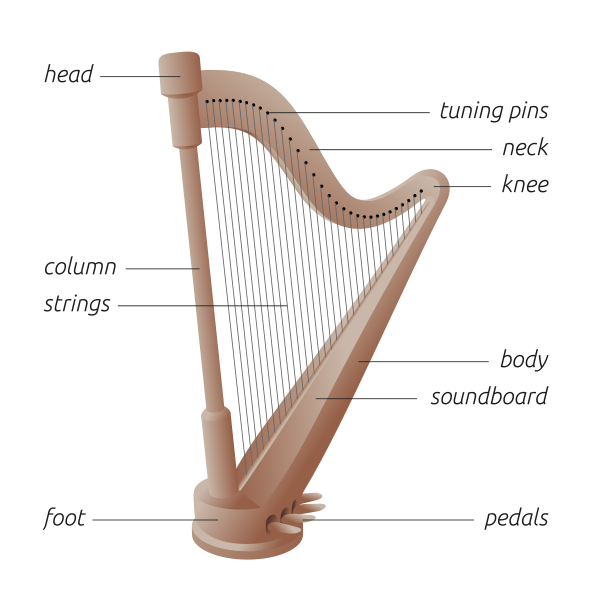
\includegraphics[width=.8\textwidth]{Harp.png}
\caption{The parts of a harp.
(Figure taken from Wikipedia.)}
\label{f:harp}
\end{center}
\end{figure}

\i The strings have fixed lengths and they are 
plucked.

\i Each string produces just one note.
(That's why a harp needs so many strings!)

\i However, by using a foot pedal that changes
the tension in the strings, one can raise or 
lower the note by a semitone.
(A harp with such a foot pedal is called a 
{\em double-action} harp.)

\ei
%%%%%%%%%%%%%%%%%%%%%%%%%%%%%%%%%%%%%%%%%%
\subsection{Guitar}
\bi

\i The guitar is probably the next simplest string
instrument.
(See Figure~\ref{f:guitar}.)
%
\begin{figure}[htbp]
\begin{center}
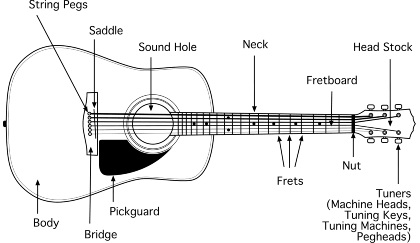
\includegraphics[width=.9\textwidth]{guitar.jpg}
\caption{The parts of a classical guitar.
(Figure taken from {\tt http://www.betterguitar.com}.)}
\label{f:guitar}
\end{center}
\end{figure}

\i It has six strings all of the same length.

\i The strings are made of different materials 
and are under different tensions, to produce notes 
with different pitches.
(The tension in the strings can be adjusted 
using the tuning keys.)

\i By pressing the strings against frets, which
are located on the neck of the guitar (between the
nut and the bridge), the effective lengths of 
the strings can be changed.
This increases the number of notes that can be 
produced.

i) By pressing a string against the seventh fret,
you decrease its length to two-thirds of its full 
length, producing a sound a perfect fifth above
that of the open string.

ii) By pressing a string against the twelfth fret,
you decrease its length to one-half of its full
length, producing a sound an octave above that of
the open string.

\i By wiggling your finger on the fretboard 
as you pluck a string, you can produce a note with a 
varying pitch.
This effect is called {\em vibrato} and is used 
especially by violinists and sometimes by vocalists.

\i The strings are coupled to the body of the 
guitar at the bridge.
The vibrations of the strings are amplified by
the body, increasing the loudness of the sound 
produced.

\ei
%%%%%%%%%%%%%%%%%%%%%%%%%%%%%%%%%%%%%%%%%%%
\subsection{Violin}
\bi

\i Although a violin looks superficially similar to a guitar, 
it differs from a guitar in many ways.
(See Figure~\ref{f:violin}.)
%
\begin{figure}[htbp]
\begin{center}
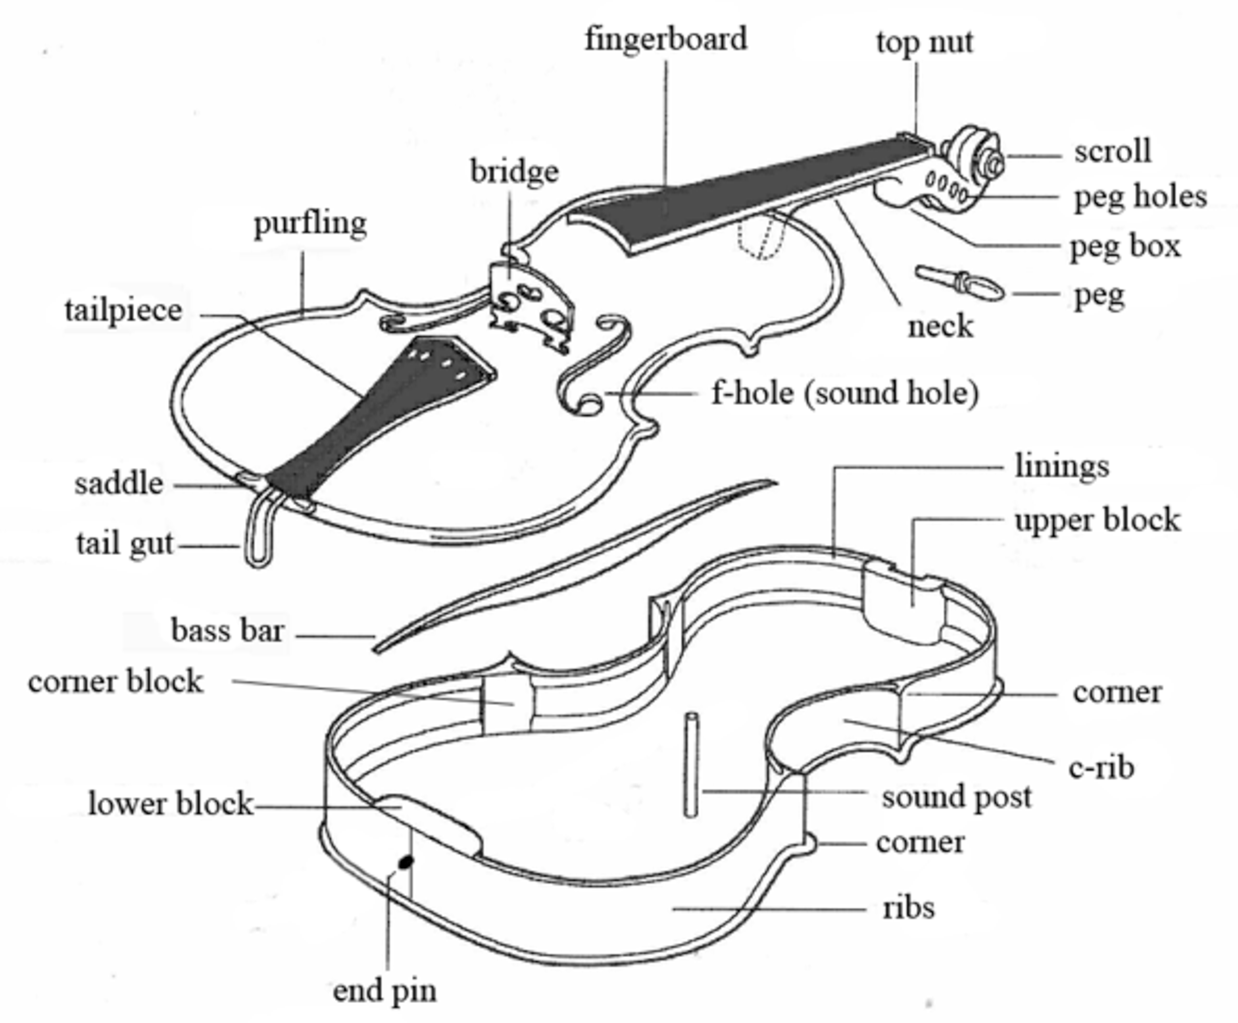
\includegraphics[width=.9\textwidth]{violin.pdf}
\caption{The parts of a violin.
(Figure taken from {\tt http://www.violinsonly.info}.)}
\label{f:violin}
\end{center}
\end{figure}

\i A violin has only four strings of fixed length
and fixed tension.
(Similar to a guitar, 
the tension in the strings can be adjusted
by using the tuning keys.)

\i Similar to a guitar, the effective length of 
the violin strings can be shortened by pressing the 
strings against the neck of the violin.
But unlike a guitar, there are no frets on a violin 
to give fixed, discrete changes in length.

\i Thus, a violin doesn't have fixed notes.
(This makes it harder for a beginner to learn
how to play a violin.)

\i The other major difference between the violin and 
the guitar is that the violin strings are bowed.
(A violinist's fingers would quickly damp 
out the vibrations of a string if it were plucked 
instead of bowed.)

\i The tone quality of a violin note can be varied by 
varying the intensity of a note while a string is being bowed.
 
\i This is in contrast to the  harp, guitar, or piano, 
where once a string is plucked or struck, nothing else can be
done to change the intensity of the note as the string vibrates.

\i The violin strings are coupled
to the body of violin at the bridge, just like a guitar.
The sound post couples the front and back of the body.

\i The sound hole of a violin (two $f$-holes)
is much smaller than the sound hole of a guitar.

\i The complex natural frequencies of the body of the 
violin and the use of a bow instead of plucking are 
two main reasons for the rich timbre of notes played on
a violin.

\ei
